\section{Model Learning}\label{modellearning}

\subsection{Mealy machines}

To model the implementation of TDLS we're going to use a specific kind of state machine, \emph{Mealy machines}. This type of state machine is a kind of deterministic finite state machine that has a transition and output for every state and input \cite{Mealy:1955}.

A Mealy machine is formed by a set of finite states (\(Q\)) and the transitions between those states. One of these states is the initial state \(q_0\), the state where the Mealy machine always starts. Transitions represent an input received while the machine is one of the its states. The transitions are defined as \(\delta : Q \times \Sigma \to Q\). This function uses the input alphabet \(\Sigma\), which is a finite set of symbols that represent the input. Different from a normal finite state machine is the output function \(\lambda = Q \times \Sigma \to \Lambda\) where \(\Lambda\) is the finite set of output symbols.

Since a Mealy machine is deterministic the state machine has only one transition for each input. This is perfect for our research since TDLS should reply the same every time the same message sequence is executed.

\begin{figure}[!h]
	\centering
	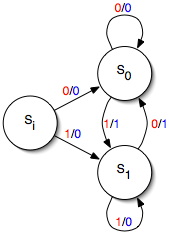
\includegraphics{mealy}
	\caption{Example of a Mealy machine}
	\label{fig:mealymachine}
\end{figure}

\subsection{Learning state machines}

Our goal is to learn a state machine of a TDLS implementation. We're approaching this by using the L* algorithm \cite{Angluin:1987}. The goal of this algorithm is to learn a finite state machine from a so-called \emph{teacher}. This teacher can be any type of computational system.
The L* algorithm is run by the learner, who tries to communicate with the teacher to infer the state machine of that teacher. In our learning process this teacher will be an implementation of TDLS.

\subsubsection{Learning process}
\label{preliminaries:learning:process}

The first step in the learning process is sending arbitrary messages to the teacher. The teacher will answer based on the message sent by the learner. These answers can differ for each type of message sent by the learner. This allows the learner to build a hypothetical state machine based on those messages, both the input and output.
Since the state machine of the learner is only hypothetical it needs needs to check with the teacher if it matches the actual state machine.

Checking if the state machines match is done by using an equivalence algorithm, in our case we choose to use \emph{randomwords}. This algorithm will send a random sequence of inputs of a predefined minimum and maximum length to the teacher. If the output of the teacher based on this input matches the inferred state machine the next sequence of input will be sent. After a predefined number of tries the learner will draw the conclusion that the inferred state machine is equal to the state machine of the teacher. If the output of the teacher does not match the state machine the learner will know based on the response, it will then try inferring a new state machine.

